\section{Introduction au problème numérique}

Les domaines de l'électromagnétisme et de l'acoustique sont régis par de nombreuses équations aux dérivées partielles faisant place à des systèmes parfois non solvables analytiquement. Cela constitue donc un défi majeur en mathématiques appliquées. Pouvoir résoudre ces équations numériquement est par conséquent essentiel à l'étude de la propagation d'un son, et donc nécessaire pour diminuer le bruit dans un réacteur d'avion.\\ \\
Dans un premier temps, nous expliquerons le problème que nous avons dû résoudre numériquement. Puis dans un second temps, nous étudierons le fonctionnement des algorithmes permettant de calculer l'énergie minimale dans le domaine. Enfin, nous analyserons les différents résultats obtenus.

\subsection{Présentation du problème}

Considérons un volume rectangulaire de 1m horizontalement et de 2m verticalement, comportant $N\times2N$ quadrangles. Le matériau poreux est déposé sur la surface au milieu, qui est plus au moins irrégulière en fonction du niveau de fractale.

\begin{figure}[H]
    \centering
    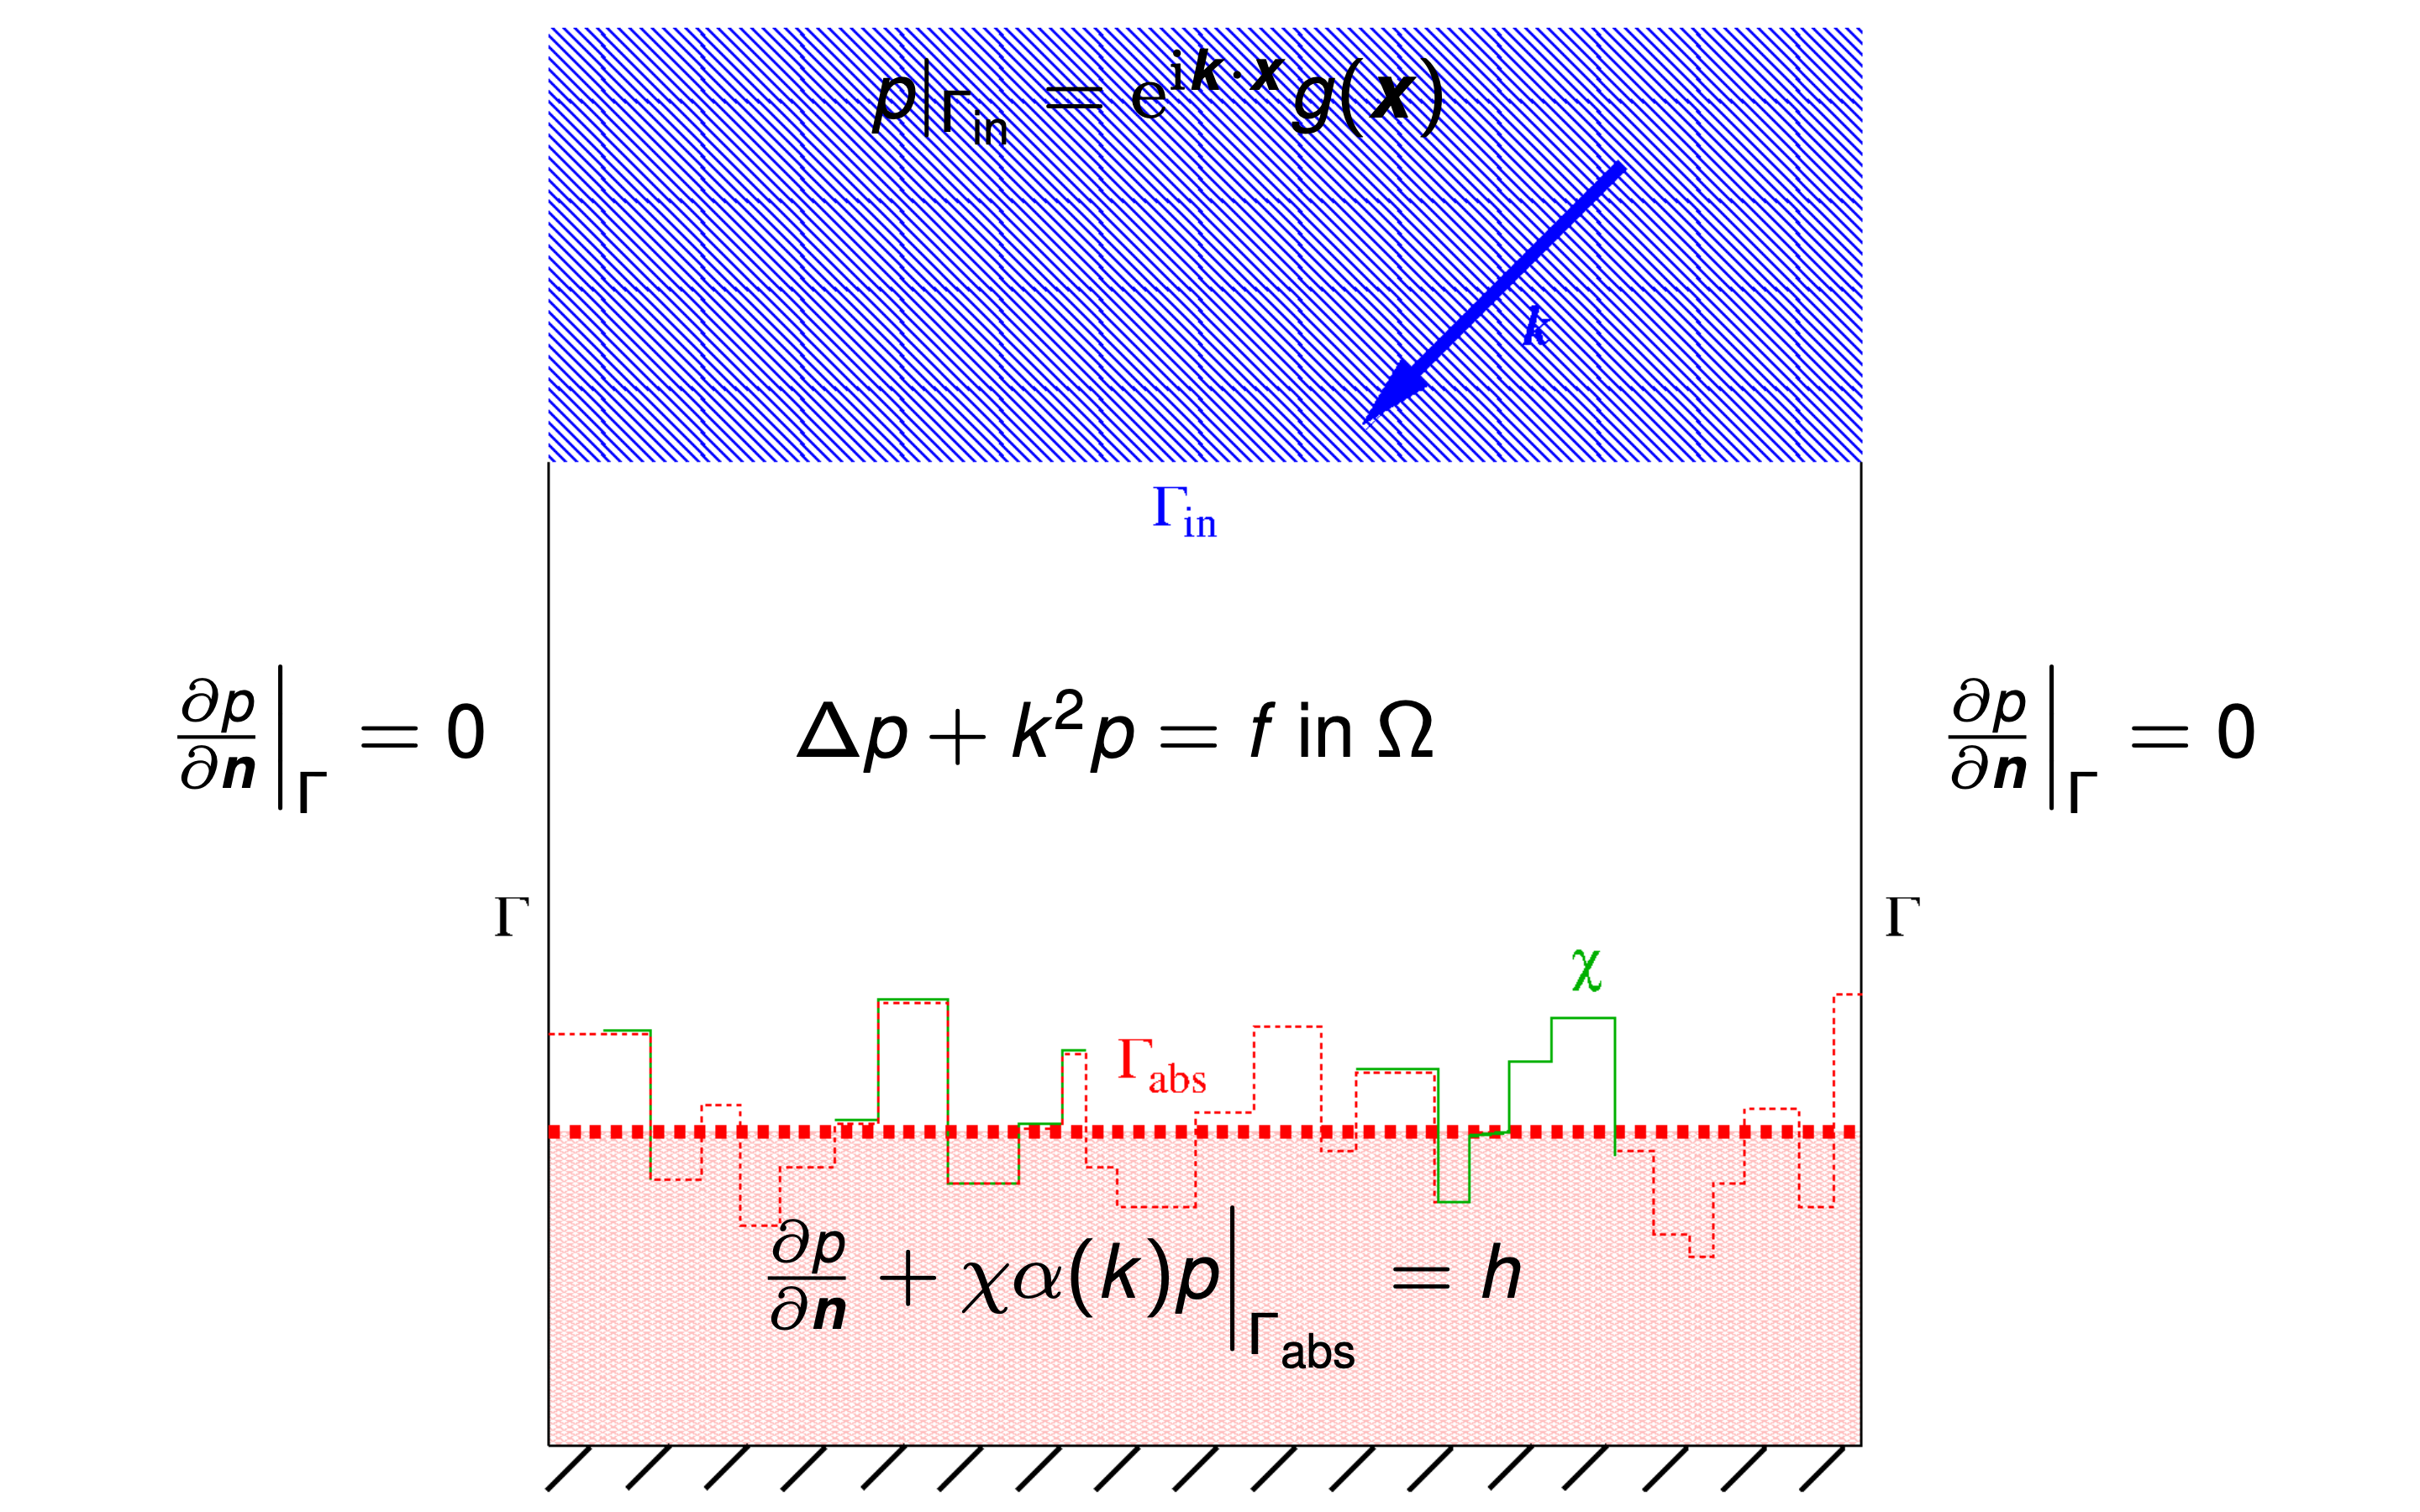
\includegraphics[width=0.8\linewidth]{rapport/numerique/assets/probleme.png}
    \caption{Modélisation du problème dans notre domaine}
    \label{fig:enter-label}
\end{figure}

On impose des conditions de Dirichlet pour la surface supérieure, des conditions de Neumann pour les surfaces latérales et des conditions de Robin pour la paroi du réacteur (surface inférieure). Le système d'équation dans le domaine est donc le suivant:
\begin{equation}
    \tag{$P_\chi$}
    \begin{cases}
    \Delta p + k^2 p = 0 \text{ dans } \Omega \\
    p = g_{in} \text{ sur } \Gamma_{in} \\
    \displaystyle \frac{\partial p}{\partial n} = 0 \text{ sur } \Gamma \\[5pt]
    \displaystyle \frac{\partial p}{\partial n} + \alpha \chi p = 0 \text{ sur } \Gamma_{abs}
    \end{cases} 
\end{equation}
où $p$ est l'inconnue du système, $\alpha$ est le coefficient d'absorption du liner et $\chi$ représente la répartition de matériaux poreux à la frontière. \\ \\
La quantité de matériaux est $$\beta = \displaystyle \displaystyle \int_{\Gamma_{abs}}\chi dS.$$
L'objectif final du projet est de trouver le niveau de fractale, le matériau et la quantité la plus faible de matériaux $\beta$ permettant de minimiser l'énergie dans le réacteur et donc le bruit dans le réacteur. \\ \\
L'énergie totale dans le domaine est donnée par la formule:
$$J(\chi) := \int_\Omega |p_\chi|^2dx$$
où $p_\chi$ est la solution du système $(P_\chi)$.

\subsection{Structure du code}

Dans le code, présent dans le fichier accompagnant ce rapport, nous trouvons cinq fichiers Python. \\ \\
Les trois premiers, \texttt{preprocessing.py}, \texttt{processing.py}, \texttt{postprocessing.py} sont des "boites noires" qui nous ont été fournies et qui n'ont pas été modifiées. Le premier fichier, \texttt{preprocessing.py} sert principalement à créer la fractale et définit des fonctions de base. Le deuxième, \texttt{processing.py}, a pour but de résoudre l'équation d'Helmholtz dans le domaine. Enfin, \texttt{postprocessing.py}, sert uniquement à créer différents graphiques montrant l'énergie dans le domaine, ou encore $\chi$, la disposition de notre matériaux poreux sur la frontière.\\ \\
L'autre fichier \texttt{\_env.py}, permet d'identifier la nature de chaque point du maillage. La liste qui traduit la nature de tous les points s'appelle \texttt{domain\_omega}, et attribue à chaque point une valeur entière non nulle entre $-2$ et $3$ en fonction de si ce point correspond à une condition de Dirichlet, de Robin, de Neumann, à l'intérieur du domaine ou à l'extérieur.\\ \\
Enfin, le dernier fichier, que nous avons complété est \texttt{main.py}. Ce fichier comporte la fonction permettant de calculer l'énergie dans le domaine et l'algorithme d'optimisation associé.
